\section{Données et pré-traitement}

\paragraph{La base.} \emph{MAP\_DATA\_WELD} \cite{mapweld,cool1996,cool1997} rassemble
des essais sur le métal déposé de soudures d'acier, tirés de 46 articles :
\textbf{1652 lignes et 44 colonnes}. Les entrées (colonnes 1 à 30) sont la composition
(21 éléments, en \% ou en ppm), les réglages de soudage (courant, tension, énergie,
procédé…) et le traitement thermique ; les sorties (31 à 43) sont des résultats
d'essais. Deux constats guident toute l'étude :
\begin{itemize}
  \item \textbf{une ligne est un essai, pas une soudure} : un même cordon occupe
    plusieurs lignes (une traction, des Charpy à plusieurs températures), soit environ
    620 cordons. Les lignes d'un même cordon ou d'un même article se ressemblent
    beaucoup, ce qui impose une évaluation regroupée par article
    (section~\ref{sec:f-protocole}) ;
  \item \textbf{chaque sortie n'est mesurée que sur une partie des lignes} : 700 à 880
    selon la grandeur. Nous prédisons les cinq sorties les mieux renseignées ; dureté,
    FATT et microstructure (moins de 140 lignes) sont écartées.
\end{itemize}

\paragraph{Valeurs manquantes.} Aucune ligne n'est complète, et les cases ne sont pas
vides au hasard (\emph{MCAR} exclu \cite{rubin1976}) : les lignes sans nickel sont à
88\,\% des soudures manuelles, contre 49\,\% pour les autres. Le traitement dépend de la
raison du manque :
\begin{itemize}
  \item \textbf{élément d'alliage jamais rapporté par un article} (Ni, Cr, Mo, V, Nb) :
    l'article ne le donne pas parce qu'il n'y en a que des traces (\emph{MNAR}). La
    médiane, tirée des aciers alliés, inventerait un acier allié : la teneur est mise à
    \textbf{0} (4278 cases) ;
  \item \textbf{valeur existante mais non rapportée} (oxygène, azote, réglages de
    soudage) : le manque s'explique par l'article (\emph{MAR}). Elle est remplacée par la
    \textbf{médiane}, avec un indicateur 0/1 « valeur manquante » ;
  \item \textbf{colonne trop vide} pour être complétée sans être inventée (Sn, As, Sb,
    Co, W, Cu, B) : elle est retirée ;
  \item \textbf{les sorties ne sont jamais complétées} : un essai non fait n'a pas de
    résultat à deviner.
\end{itemize}

\paragraph{Autres traitements.} Les nombres écrits en texte sont convertis (« <0,01 »
devient 0,01 ; des ppm notés en \% sont corrigés). Les variables catégorielles
(procédé, type de courant, polarité) sont encodées en \emph{one-hot}, après regroupement
des procédés rares en cinq familles. La température du traitement thermique est gardée
comme nombre, complétée de deux indicateurs « soudure brute » et « dégazage » : lue
seule, elle ferait du dégazage (\SI{250}{\celsius}) un demi-revenu. Les valeurs extrêmes
sont conservées : examinées une à une, ce sont des soudures réelles et rares, sauf un
essai Charpy à \SI{188}{\celsius}, erreur de saisie retirée. Les mesures répétées
(mêmes entrées, mêmes conditions d'essai) sont fusionnées par leur moyenne. Enfin, les
variables sont standardisées pour les modèles sensibles à l'échelle (linéaires, ACP),
pas pour les arbres.

\paragraph{Relations entre variables.} La corrélation de Spearman, peu sensible aux
valeurs extrêmes, associe les éléments d'alliage à plus de résistance et moins de
ductilité ; l'énergie Charpy dépend surtout de la température d'essai ($r = 0{,}46$).
L'ACP (figure~\ref{fig:f-acp}) montre que \textbf{les entrées sont peu redondantes} :
deux axes n'expliquent que 38\,\% de la variance, et nous gardons toutes les variables.
L'axe 1 oppose aciers alliés et traités thermiquement aux aciers ordinaires : alliage et
traitement varient ensemble, et leurs effets ne pourront pas être séparés. L'axe 2
correspond à la chaleur apportée par le soudage (arc submergé contre arc manuel).

\begin{figure}[!htbp]
  \centering
  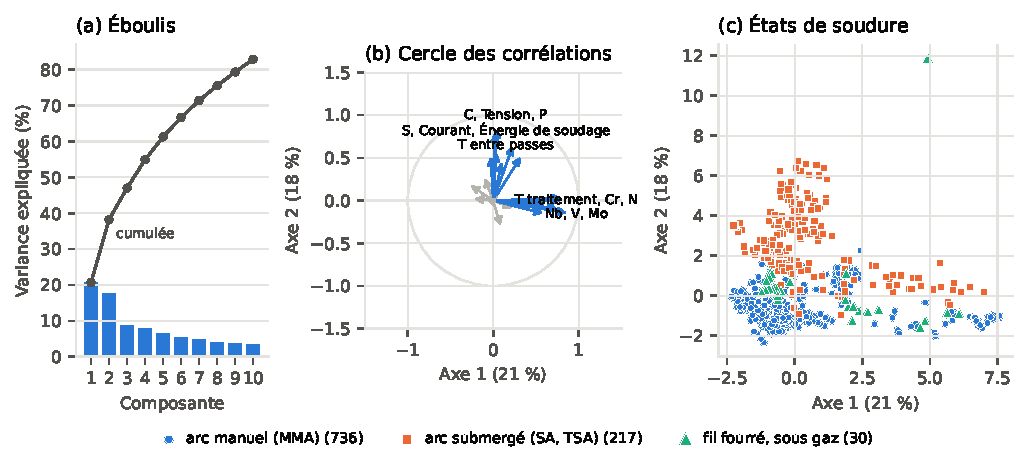
\includegraphics[width=\linewidth]{acp}
  \caption{ACP des 20 entrées numériques (983 combinaisons d'entrées distinctes,
    standardisées) : (a) variance expliquée, (b) cercle des corrélations (en bleu, les
    variables bien représentées), (c) projection des soudures par famille de procédé.}
  \label{fig:f-acp}
\end{figure}
